\documentclass[10pt,a4paper]{article}
\usepackage[margin=22mm]{geometry}
\usepackage[T1]{fontenc}
\usepackage{lmodern,microtype,booktabs,tabularx,xcolor,enumitem,amsmath}
\usepackage{tikz}
\usetikzlibrary{arrows.meta,positioning,calc,fit}
\usepackage[colorlinks=true,linkcolor=blue!50!black]{hyperref}
\setlist{itemsep=1pt,topsep=3pt}
\newcommand{\code}[1]{\texttt{#1}}
\newcommand{\meas}{\textsuperscript{M}}
\newcommand{\est}{\textsuperscript{E}}
\title{\textbf{Gust N1 v0.1}\\[2pt]\large A Linux-capable processor grown from the Gust microcontroller core\\Architecture plan and stage 1 report (spec v1)}
\author{Designed for Allan \quad$\cdot$\quad 15 November 2026}
\date{}
\begin{document}
\maketitle
\noindent\fbox{\parbox{0.97\linewidth}{\small
\textbf{What this is.} Gust N1 is the ``computer'' branch of Gust: the same core, extended step by step until it can run Linux. This document is the plan for all five stages and the report for \textbf{stage 1, which is built and tested}: user and supervisor privilege modes and a memory-management unit. Stages 2--5 are specified here but \textbf{not built}.

\meas{} = measured in this project (simulation or Yosys). \est{} = my estimate. Nothing has run on an FPGA; Linux has not been booted.}}

\section{Where N1 stands after stage 1}
\begin{center}\small\begin{tabular}{@{}ll@{}}\toprule
ISA & RV32IMC + Zicsr + Zifencei + Zba/Zbb/Zbs + Zcb, privilege levels M, S and U \\
Virtual memory & Sv32: 4\,KiB pages and 4\,MiB superpages, hardware page-table walker, 8-entry TLB \\
Tests & 294 of 294 pass\meas{} (each program on ideal and on randomly stalling buses) \\
Reuse & 5 Gust modules unchanged, 3 lightly modified, 1 rewritten, 2 new (table~\ref{tab:reuse}) \\
Core area & 20\,817 cells, 0.162\,mm$^2$ in SkyWater 130\meas{} (Gust: 16\,315 cells, 0.122\,mm$^2$) \\
Logic depth & 11.2\,ns typical\meas{} (Gust: 8.0\,ns); the TLB lookup sits in the address path \\
Can it run Linux? & \textbf{Not yet.} It still lacks atomics, large memory, caches and boot firmware (stages 2--4) \\
\bottomrule\end{tabular}\end{center}

\section{What ``turning Gust into a computer'' means}
A microcontroller runs one trusted program directly on the hardware. A computer runs an operating system that gives every program its own private address space and can stop a misbehaving program without crashing. Four things make that possible, and Gust v1.0 had none of them:
\begin{enumerate}
\item \textbf{Privilege levels} so the OS (supervisor) is protected from programs (user), with firmware (machine) below both.
\item \textbf{Virtual memory}: a memory-management unit translates each program's addresses through page tables.
\item \textbf{Much more memory} than fits on the chip, with caches to hide how slow it is.
\item \textbf{Atomic instructions}, which the Linux kernel requires.
\end{enumerate}
Stage 1 delivers the first two, which are the invasive ones: they change what every instruction and every memory access is allowed to do.

\paragraph{Honest ceiling.} N1 will be a real, small Linux computer, comparable in spirit to an early-1990s workstation at tens of MHz. It will not approach a Raspberry Pi 5, which needs 64-bit out-of-order cores and a 16\,nm process.

\section{How Gust was reused}\label{sec:reuse}
\begin{table}[h]\centering\small
\begin{tabular}{@{}llp{78mm}@{}}\toprule
Module & Status & What changed \\\midrule
\code{gust\_rvc}, \code{gust\_alu}, \code{gust\_muldiv}, & \textbf{unchanged} & byte-identical to Gust v1.0\meas \\
\code{gust\_regfile}, \code{gust\_icg} & & \\
\code{gust\_fetch} & +11 lines\meas & carries a ``page fault'' flag with each parcel and reports which half of an instruction faulted \\
\code{gust\_decode} & +11 lines\meas & decodes \code{sret} and \code{sfence.vma} \\
\code{gust\_core} & +67 / $-$15 lines\meas & privilege checks on instructions, cause codes by privilege, page-fault causes, redirect on \code{sret}/\code{sfence.vma}/\code{satp} writes, context outputs for the MMU \\
\code{gust\_csr} & rewritten, 434 lines & privilege register; \code{mstatus} S-mode fields; \code{medeleg}/\code{mideleg}; all supervisor CSRs; \code{satp}; counter enables; access checks. Counters and debug CSRs kept \\
\code{gust\_mmu} & \textbf{new}, 268 lines & TLB, page-table walker, permission checks \\
\code{n1\_core} & \textbf{new}, 99 lines & wrapper: core + MMU, same ports as \code{gust\_core} \\\bottomrule
\end{tabular}
\caption{Reuse of the Gust v1.0 core in N1 stage 1.}\label{tab:reuse}
\end{table}
The Gust SoC (bus, RAM, boot ROM, UART, SPI, GPIO, timers, JTAG debug) is untouched and \code{n1\_core} has the same ports as \code{gust\_core}, so it drops straight into \code{gust\_soc}. That integration has not been run yet.

\paragraph{The idea that made reuse possible.} Gust already had precise bus errors: a failed fetch or data access comes back as an error response and the core turns it into an exact trap. In N1 the MMU sits \emph{between} the core and the buses and reports a page fault as that same error response, with one extra wire saying ``this one is a page fault''. The pipeline, hazard logic and trap timing therefore did not have to be redesigned.

\begin{center}
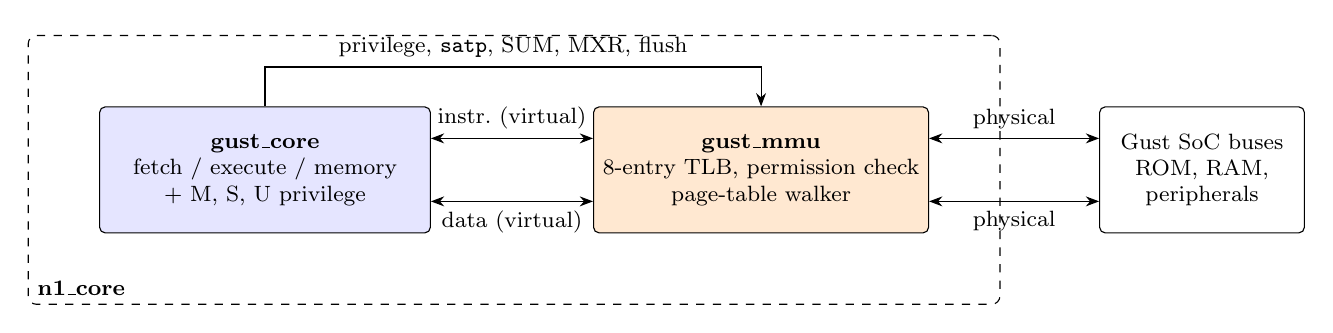
\begin{tikzpicture}[font=\footnotesize,b/.style={draw,rounded corners=2pt,minimum height=10mm,align=center},>=Stealth]
\node[b,fill=blue!10,minimum width=42mm,minimum height=16mm] (core) at (0,0) {\textbf{gust\_core}\\fetch / execute / memory\\+ M, S, U privilege};
\node[b,fill=orange!18,minimum width=40mm,minimum height=16mm] (mmu) at (6.3,0) {\textbf{gust\_mmu}\\8-entry TLB, permission check\\page-table walker};
\node[b,minimum width=26mm,minimum height=16mm] (bus) at (11.9,0) {Gust SoC buses\\ROM, RAM,\\peripherals};
\draw[<->] ($(core.east)+(0,4mm)$) -- node[above]{instr.\ (virtual)} ($(mmu.west)+(0,4mm)$);
\draw[<->] ($(core.east)+(0,-4mm)$) -- node[below]{data (virtual)} ($(mmu.west)+(0,-4mm)$);
\draw[<->] ($(mmu.east)+(0,4mm)$) -- node[above]{physical} ($(bus.west)+(0,4mm)$);
\draw[<->] ($(mmu.east)+(0,-4mm)$) -- node[below]{physical} ($(bus.west)+(0,-4mm)$);
\draw[->] (core.north) -- ++(0,5mm) -| node[pos=0.25,above]{privilege, \code{satp}, SUM, MXR, flush} (mmu.north);
\node[draw,dashed,rounded corners=3pt,fit=(core)(mmu),inner sep=9mm,label={[anchor=south west]south west:\textbf{n1\_core}}] {};
\end{tikzpicture}
\end{center}

\section{Stage 1 design}
\subsection{Privilege}
\begin{itemize}
\item Three levels: machine (3), supervisor (1), user (0). Reset enters machine mode, as before.
\item Traps go to machine mode unless delegated with \code{medeleg} (exceptions) or \code{mideleg} (interrupts), in which case they enter supervisor mode through \code{stvec} with \code{sepc}, \code{scause}, \code{stval}.
\item \code{mret} and \code{sret} restore the previous privilege from MPP and SPP. \code{ecall} raises cause 8, 9 or 11 by privilege.
\item Illegal below their level: \code{mret}, \code{sret}, \code{wfi}, \code{sfence.vma} and any CSR whose address encodes a higher privilege. TSR, TVM and TW let firmware trap \code{sret}, \code{satp}/\code{sfence.vma} and \code{wfi} from supervisor mode. \code{mcounteren}/\code{scounteren} gate the cycle and instruction counters.
\item Supervisor interrupts: SSIP, STIP, SEIP are software-set bits (firmware injects timer and external interrupts this way). Machine interrupts always win; a delegated interrupt is never taken in machine mode.
\item Debug mode runs with machine privilege; the interrupted level is saved in \code{dcsr.prv} and restored on resume.
\end{itemize}

\subsection{Memory-management unit}
\begin{itemize}
\item \textbf{Translation off} (machine mode, or \code{satp.MODE}=0): pure wires, no added cycle. Gust-style firmware runs exactly as before.
\item \textbf{TLB hit:} the request leaves in the same cycle with the translated address. One shared 8-entry fully associative TLB serves fetches and data.
\item \textbf{TLB miss:} the request is held while the walker reads one or two page-table entries through the data bus (about 2--4 extra cycles with on-chip memory), then retried.
\item \textbf{Permissions} R, W, X, U and the SUM and MXR bits are checked on every access from the cached entry. \code{mstatus.MPRV} applies to data accesses.
\item \textbf{Accessed/dirty bits} are never written by hardware. An access that needs A or D set raises a page fault and the OS sets the bit. This is the simpler of the two behaviours the RISC-V specification allows, and Linux supports it.
\item \textbf{Faults:} cause 12, 13 or 15. The fault address is exact; for an instruction that straddles two pages it names the page that is missing, which an OS needs for demand paging.
\item \textbf{Flushing:} no address-space IDs. A write to \code{satp} or \code{sfence.vma} empties the TLB and refetches the following instructions. A permission fault drops the offending entry, so a retry sees the updated page table.
\item \textbf{Context changes:} no fetch request is issued in the cycle a trap, return or \code{satp} write takes effect, so nothing is ever fetched with stale privilege. Cost: one extra cycle per trap or return.
\end{itemize}

\section{Stage 1 verification\meas}
\begin{center}\small\begin{tabularx}{\linewidth}{@{}lXr@{}}\toprule
Group & What it checks & Programs \\\midrule
Gust regression & the 90 machine-mode ISA tests from Gust v1.0, unchanged: nothing that worked broke & 90 \\
\code{rv32si} & supervisor CSRs, \code{scall}, \code{sbreak}, \code{wfi}, misaligned fetch, accessed/dirty bits with MPRV & 6 \\
\code{rv32ui/um/uc-v} & every base, multiply and compressed instruction test re-run in \textbf{user mode under Sv32 paging}, with a small supervisor kernel that maps pages on demand & 50 \\
\code{n1-directed-priv} & written for N1: illegal instructions and CSRs by privilege, TSR/TVM/TW, counter enables, delegated and non-delegated supervisor timer interrupt, SUM, MXR, read-only pages, \code{sfence.vma}, misaligned superpage, page-straddling instruction & 1 \\\midrule
& each program on ideal and on randomly stalling buses: \textbf{294 runs, all pass}; also all pass with clock gating enabled & 147 \\\bottomrule
\end{tabularx}\end{center}
\textbf{The tests can fail.} Four deliberately injected bugs were each caught: wrong fault address for a straddling instruction, ignoring the U bit, never delegating interrupts, skipping the dirty-bit check.

\textbf{One real bug was found and fixed:} the page-table walker could put a request on the data bus while an earlier response was still outstanding. It only showed with randomly stalling buses.

\textbf{Not covered:} the official architectural compliance suite, formal verification, random instruction streams under paging, debug mode together with paging, and \code{n1\_core} inside the SoC.

\section{Cost of stage 1\meas}
\begin{center}\small\begin{tabular}{@{}lrrr@{}}\toprule
 & Gust v1.0 core & N1 stage 1 core & Change \\\midrule
Cells (SkyWater 130, flattened) & 16\,315 & 20\,817 & +28\% \\
Cell area & 0.122\,mm$^2$ & 0.162\,mm$^2$ & +33\% \\
Flip-flops & 1\,756 & 2\,423 & +38\% \\
Logic depth, typical corner & 8.0\,ns & 11.2\,ns & +39\% \\\bottomrule
\end{tabular}\end{center}
Of the increase, the MMU is 2\,846 cells (0.025\,mm$^2$) and the larger CSR block about 0.010\,mm$^2$. The longer logic depth is the price of translating in the same cycle as the access; stage 3 removes it. CoreMark was not re-measured: in machine mode the MMU adds no cycles, so it should be unchanged at 2.93 CoreMark/MHz\est.

\section{The remaining stages (not built)}
\begin{center}\small\begin{tabularx}{\linewidth}{@{}cp{27mm}Xp{27mm}@{}}\toprule
Stage & Adds & Why it is needed / what is reused & Done when \\\midrule
1 & M/S/U, Sv32 MMU & this document & \textbf{done} \\
2 & A extension (\code{lr/sc}, \code{amo*}); interrupt controller (PLIC) & Linux requires atomics. One hart, so \code{amo} is a read-modify-write in the existing memory stage. The Gust bus and peripherals are reused as they are & \code{rv32ua} tests pass \\
3 & External memory + caches & 32\,MiB or more of SDRAM or PSRAM on the FPGA board, behind instruction and data caches. The TLB lookup moves alongside the cache lookup, which restores the clock rate & memory test + CoreMark from external RAM \\
4 & Boot software & OpenSBI firmware in machine mode (it emulates the \code{time} CSR and anything missing), a device tree, a kernel built for \code{rv32ima} with a RAM disk. The Gust UART is the console & Linux prints a shell prompt on the FPGA \\
5 & Second core (optional) & two \code{n1\_core} instances; needs real atomics across cores and inter-processor interrupts. This is the only place where ``stacking'' cores pays off & Linux reports 2 CPUs \\\bottomrule
\end{tabularx}\end{center}
\paragraph{Board for stages 3--4.} The Tang Nano 20K has only 8\,MiB of SDRAM, which is too little for a comfortable Linux boot\est. Plan on an FPGA board with at least 32\,MiB of SDRAM (for example a ULX3S) or add a PSRAM module. Verify the memory size of whichever board you choose.
\paragraph{Why Linux cannot be proven in simulation here.} A boot is on the order of a billion instructions\est: hours of simulation and no way to check it cheaply. The standard practice is to simulate the first milliseconds of boot, then move to the FPGA.

\section{Known limitations of stage 1}
\begin{itemize}
\item No atomics, no caches, no external memory, no interrupt controller: cannot boot Linux yet.
\item No address-space IDs, so every address-space switch empties the 8-entry TLB. Fine for correctness, slow for multitasking; stage 3 should enlarge the TLB and add ASIDs.
\item No physical memory protection (PMP). Machine-mode firmware is not protected from supervisor mode by hardware; OpenSBI tolerates this, a security-minded design would not.
\item Logic depth rose 39\%. Until stage 3, expect a proportionally lower clock.
\item The page-table walker shares the data bus and stalls the data port while it runs.
\item \code{mtval} is zero for illegal instructions (allowed; firmware then reads the instruction itself).
\item Physical addresses are 32 bits; a page-table entry pointing above 4\,GiB raises an access fault.
\end{itemize}

\section{Files and how to run}
\begin{center}\small\begin{tabular}{@{}ll@{}}\toprule
\code{rtl/} & the 11 core files: \code{n1\_core.v}, \code{gust\_mmu.v}, \code{gust\_csr.v} and the reused Gust files \\
\code{tb/} & core test bench, test builder, \code{sw/n1\_priv.c} (directed test), Makefile \\\bottomrule
\end{tabular}\end{center}
\begin{quote}\small\code{cd tb \&\& make prepare RISCV\_TESTS=/path/to/riscv-tests \&\& make}\end{quote}
Needs the same tools as Gust, plus C library headers for the test kernel (picolibc; the builder's \code{--libc-include} option sets the path). Expect \code{TESTS=294 PASS=294} twice, about six minutes each.
\end{document}
